%!TEX root = bare_conf.tex

\begin{figure}[!t]
	\centering
	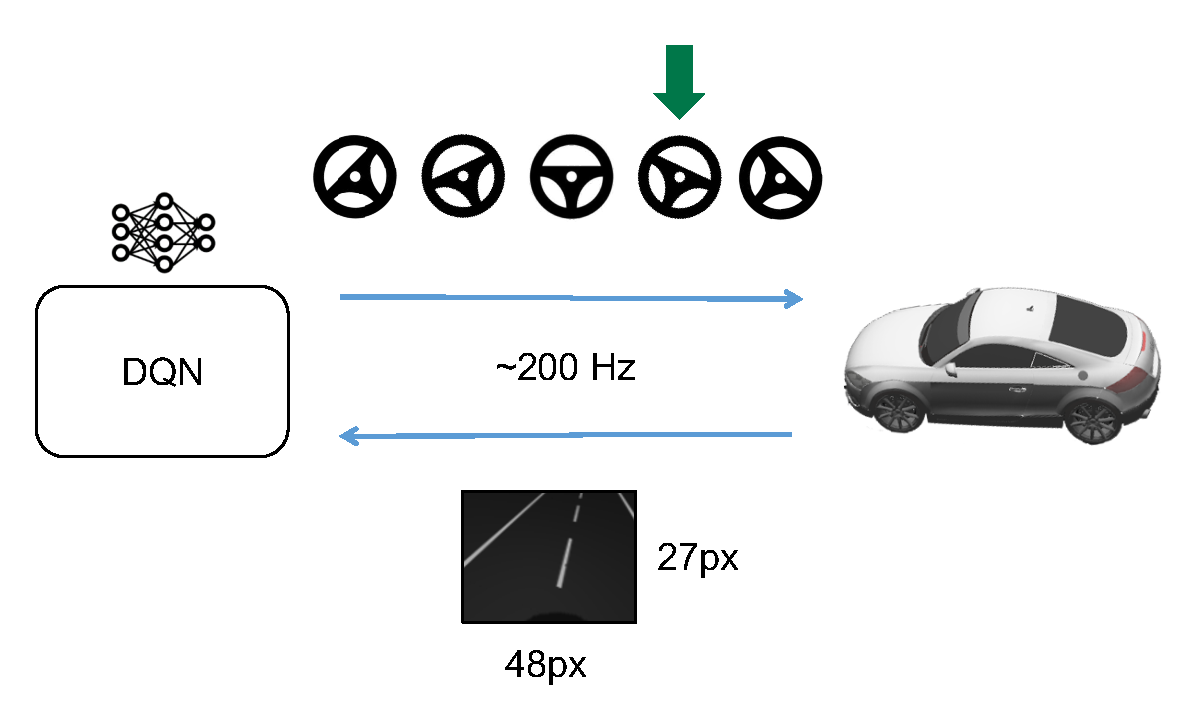
\includegraphics[width=3.5in]{../presentation/archi} 
	\vspace{-2.5em}
	\caption{System architecture: Every time the simulation (depicted as vehicle) sends a camera image to DQN, a set of Q-values are calculated by the net, one for each action. The action corresponding to the largest Q-value is selected. As an example here the action: \textit{Half-right} is selected.}
	\label{fig:archi}
\end{figure}

\section{Setup} \label{sec:setup}
Gazebo\footnote{\url{http://gazebosim.org}} was used as the simulation environment. We had one car model and a small tileset of track pieces at our disposal to build custom tracks. The car was almost as wide as an entire lane, which made the task even more challenging. We were given plug-ins, which simplified the controls to setting a speed value in $[-1, 1]$ and a steering angle in $[-1, 1]$. This led to our action set, listed in section \ref{actionset}.

We selected Caffe\cite{jia2014caffe} as deep learning framework and Ros \footnote{\url{http://www.ros.org}} was chosen as a tool for the communication between DQN and Gazebo.